%%%%%%%%%%%%%%%%%%%%%%%%%%%%%%%%%%%%%%%%%%%%%%
%                insertmeeting
% 1) Title (something creative & funny?)
% 2) Date (MM/DD/YYYY)
% 3) Location (ex. Hagerty High School)
% 4) People/Committees Present 
% 5) Picture 
% 6) Start Time & Stop Time (ex. 12:30AM to 4:30PM)
%%%%%%%%%%%%%%%%%%%%%%%%%%%%%%%%%%%%%%%%%%%%%%
\insertmeeting 
	{Slippery Software} 
	{11/01/21}
	{Hagerty High School}
	{Anouska, Jensen, Nathan, Ritam, Samantha}
	{Images/RobotPics/robot.jpg}
	{2:30 - 6:30}
	
\hhscommittee{Software}
\noindent\hfil\rule{\textwidth}{.4pt}\hfil
\subsubsection*{Goals}
\begin{itemize}
    \item To add the Carousel class and get it working
    \item To make the arm more stable with software

\end{itemize} 

\noindent\hfil\rule{\textwidth}{.4pt}\hfil

\subsubsection*{Accomplishments}
Hooray! It’s the first day of November and I personally love when it gets to the cold part of the year. Anyways, today we worked on a lot of the beginning stages of programming our mechanisms. We created a Carousel class to main object oriented style programming and quickly found that 1.0 power on the 6000 RPM motor we decided to use was a little too fast. Now, you might be wondering why we decided to use that 6000 RPM motor, but without the gearbox, it would allow the robot to be lighter, allowing us to be faster. More on that is written about in the hardware section. Back to programming the carousel, we figured out that we needed to find a quick way to test the powers without redownloading the code to test the different powers. As a result, we found a solution by using the joystick to spin the carousel until we get the power we want it to be at. We then had a button for which when it was pressed, the carousel power would be stored in a variable. We would then print the variable to the screen and it would show what power we needed the carousel to be at. Pictures of our code are shown below. After working on the carousel, we worked on stabilizing the arm a bit. At first we tried a PID controller, however since the powers we needed were not linear, this did not really work too well, as we needed less power when it reached towards the center. We then tried an array of powers, for when it was in a certain position, it would be set to a certain power. This didn’t really work too well and it would cause the arm to be shaky. After that we just said if the position is greater than 0 (the starting position), then we would set the target to 0, and if it was past 0 to let the arm just fall so the block doesn’t come out of our grabber. This happened to be a lot better, however sometimes the block would still come out. As a solution, we plan on using the sine function to help put a negative power to counteract gravity when the arm is falling. This will allow the arm to fall really slowly. 

 

\begin{figure}[ht]
\centering
\begin{minipage}[b]{.48\textwidth}
  \centering
  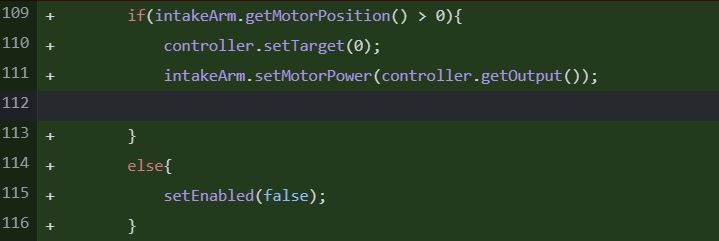
\includegraphics[width=0.95\textwidth]{Meetings/November/11-01-21/armMonday1 - Ritam R.JPG}
  \caption{Intake arm code.}
  \label{fig:pic1}
\end{minipage}%
\hfill%
\begin{minipage}[b]{.48\textwidth}
  \centering
  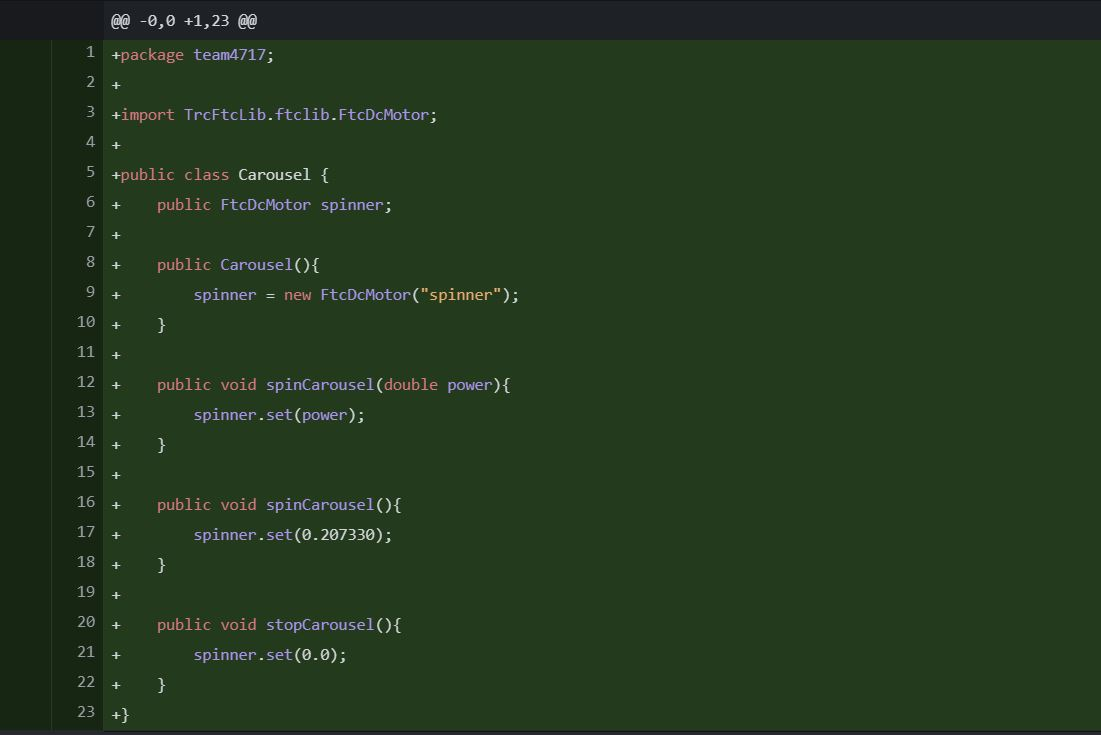
\includegraphics[width=0.95\textwidth]{Meetings/November/11-01-21/carousel1 - Ritam R.JPG}
  \caption{Our new Carousel spinner class.}
  \label{fig:pic2}
\end{minipage}
\end{figure}

\begin{figure}[htp]
\centering
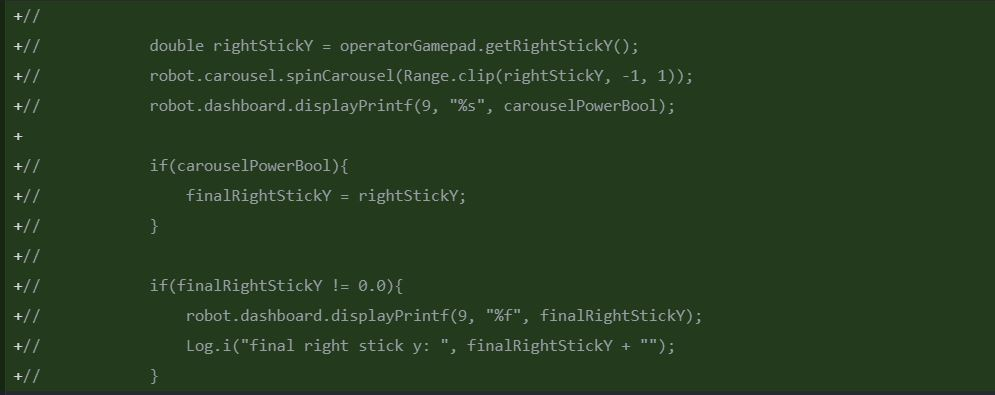
\includegraphics[width=0.95\textwidth, angle=0]{Meetings/November/11-01-21/carousel2 - Ritam R.JPG}
\caption{Our tele-op controls for the carousel.}
\label{fig:pic3}
\end{figure}

\hhscommittee{Hardware}
\noindent\hfil\rule{\textwidth}{.4pt}\hfil
\subsubsection*{Goals}
\begin{itemize}
    \item Create a part to protect robot’s front wheel
    \item Learn to use sheet metal tools in CAD and at the innovation lab
\end{itemize} 

\noindent\hfil\rule{\textwidth}{.4pt}\hfil

\subsubsection*{Accomplishments}
As meet 1 draws closer and closer, we have started to assess the robots competition practicality and less about its potential for the future. One thing that needs to be improved is the robots resilience, especially at the front of the robot. One of the most important parts of the robot, its front wheel, is also its weakest point. Being the robot’s sole component for movement, we need to do a better job protecting it from collisions with the wall or other robots. Instead of using 3d printed or laser cut parts, both of which might not be strong enough to withstand a direct collision with a wall, we decided to use folded sheet metal. 
Because this is a new way of creating parts for us, we had to learn how to use the necessary tools for the job. Much like most of our other parts, the front bumper started in CAD. We were able to quickly learn how to use onshape’s sheet metal tools, creating a simple bumper with a 90 degree flange to add support (Figure \ref{fig:pic4}). Onshape then provided us with a flattened version of the bumper that we can use as a template to cut out then fold into the proper shape (Figure \ref{fig:pic5}).
To take the bumper from CAD into the real world, we used the template generated by onshape and laser cut it out of some 1/8 inch wood. This gave us something to trace the notches around and made it easier to mark the spots where we need to bend the sheet metal. Using a shear in the UCF innovation lab (Figure \ref{fig:pic6}), our mentor showed us how to cut sheet metal. Once the 1/16 inch sheet metal was cut down into the basic rectangular shape of the bumper, we used a dremel to add the slices that would allow us to bend the bottom into a flange. With the metal cut into the correct flat shape, we used a brake to make all of the bends in the bumper (Figure \ref{fig:pic7}). The final product was an exact replica of what we created in CAD (Figure \ref{fig:pic8}). We plan on adding this part to the robot at the next meeting. We will attach the bumper to the drivetrain by drilling holes in the plastic and screwing it in using nuts and bolts.

\begin{figure}[ht]
\centering
\begin{minipage}[b]{.48\textwidth}
  \centering
  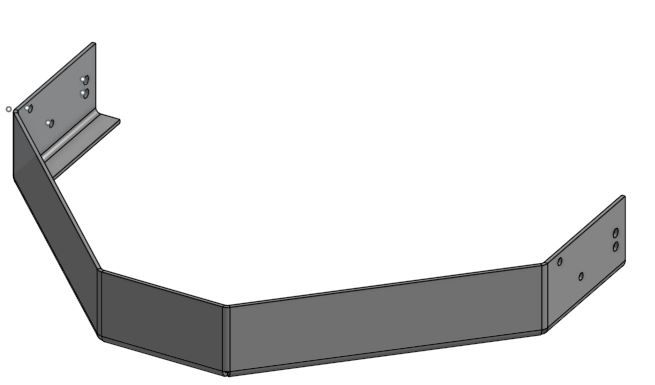
\includegraphics[width=0.95\textwidth]{Meetings/November/11-01-21/11-1-21_Hardware_Figure1 - Nathan Forrer.JPG}
  \caption{Bumper with flange}
  \label{fig:pic4}
\end{minipage}%
\hfill%
\begin{minipage}[b]{.48\textwidth}
  \centering
  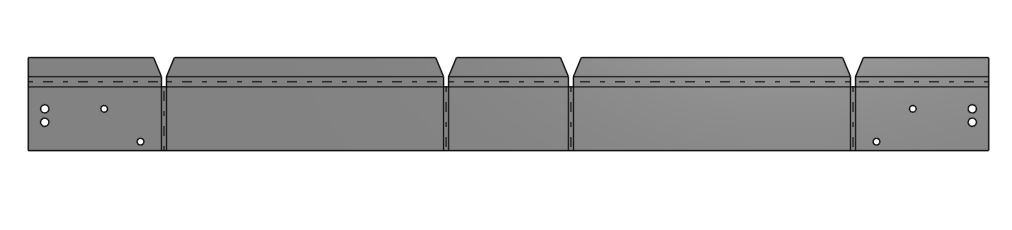
\includegraphics[width=0.95\textwidth]{Meetings/November/11-01-21/11-1-21_Hardware_Figure2 - Nathan Forrer.JPG}
  \caption{The bumper net created with Onshape}
  \label{fig:pic5}
\end{minipage}
\end{figure}

\begin{figure}[ht]
\centering
\begin{minipage}[b]{.48\textwidth}
  \centering
  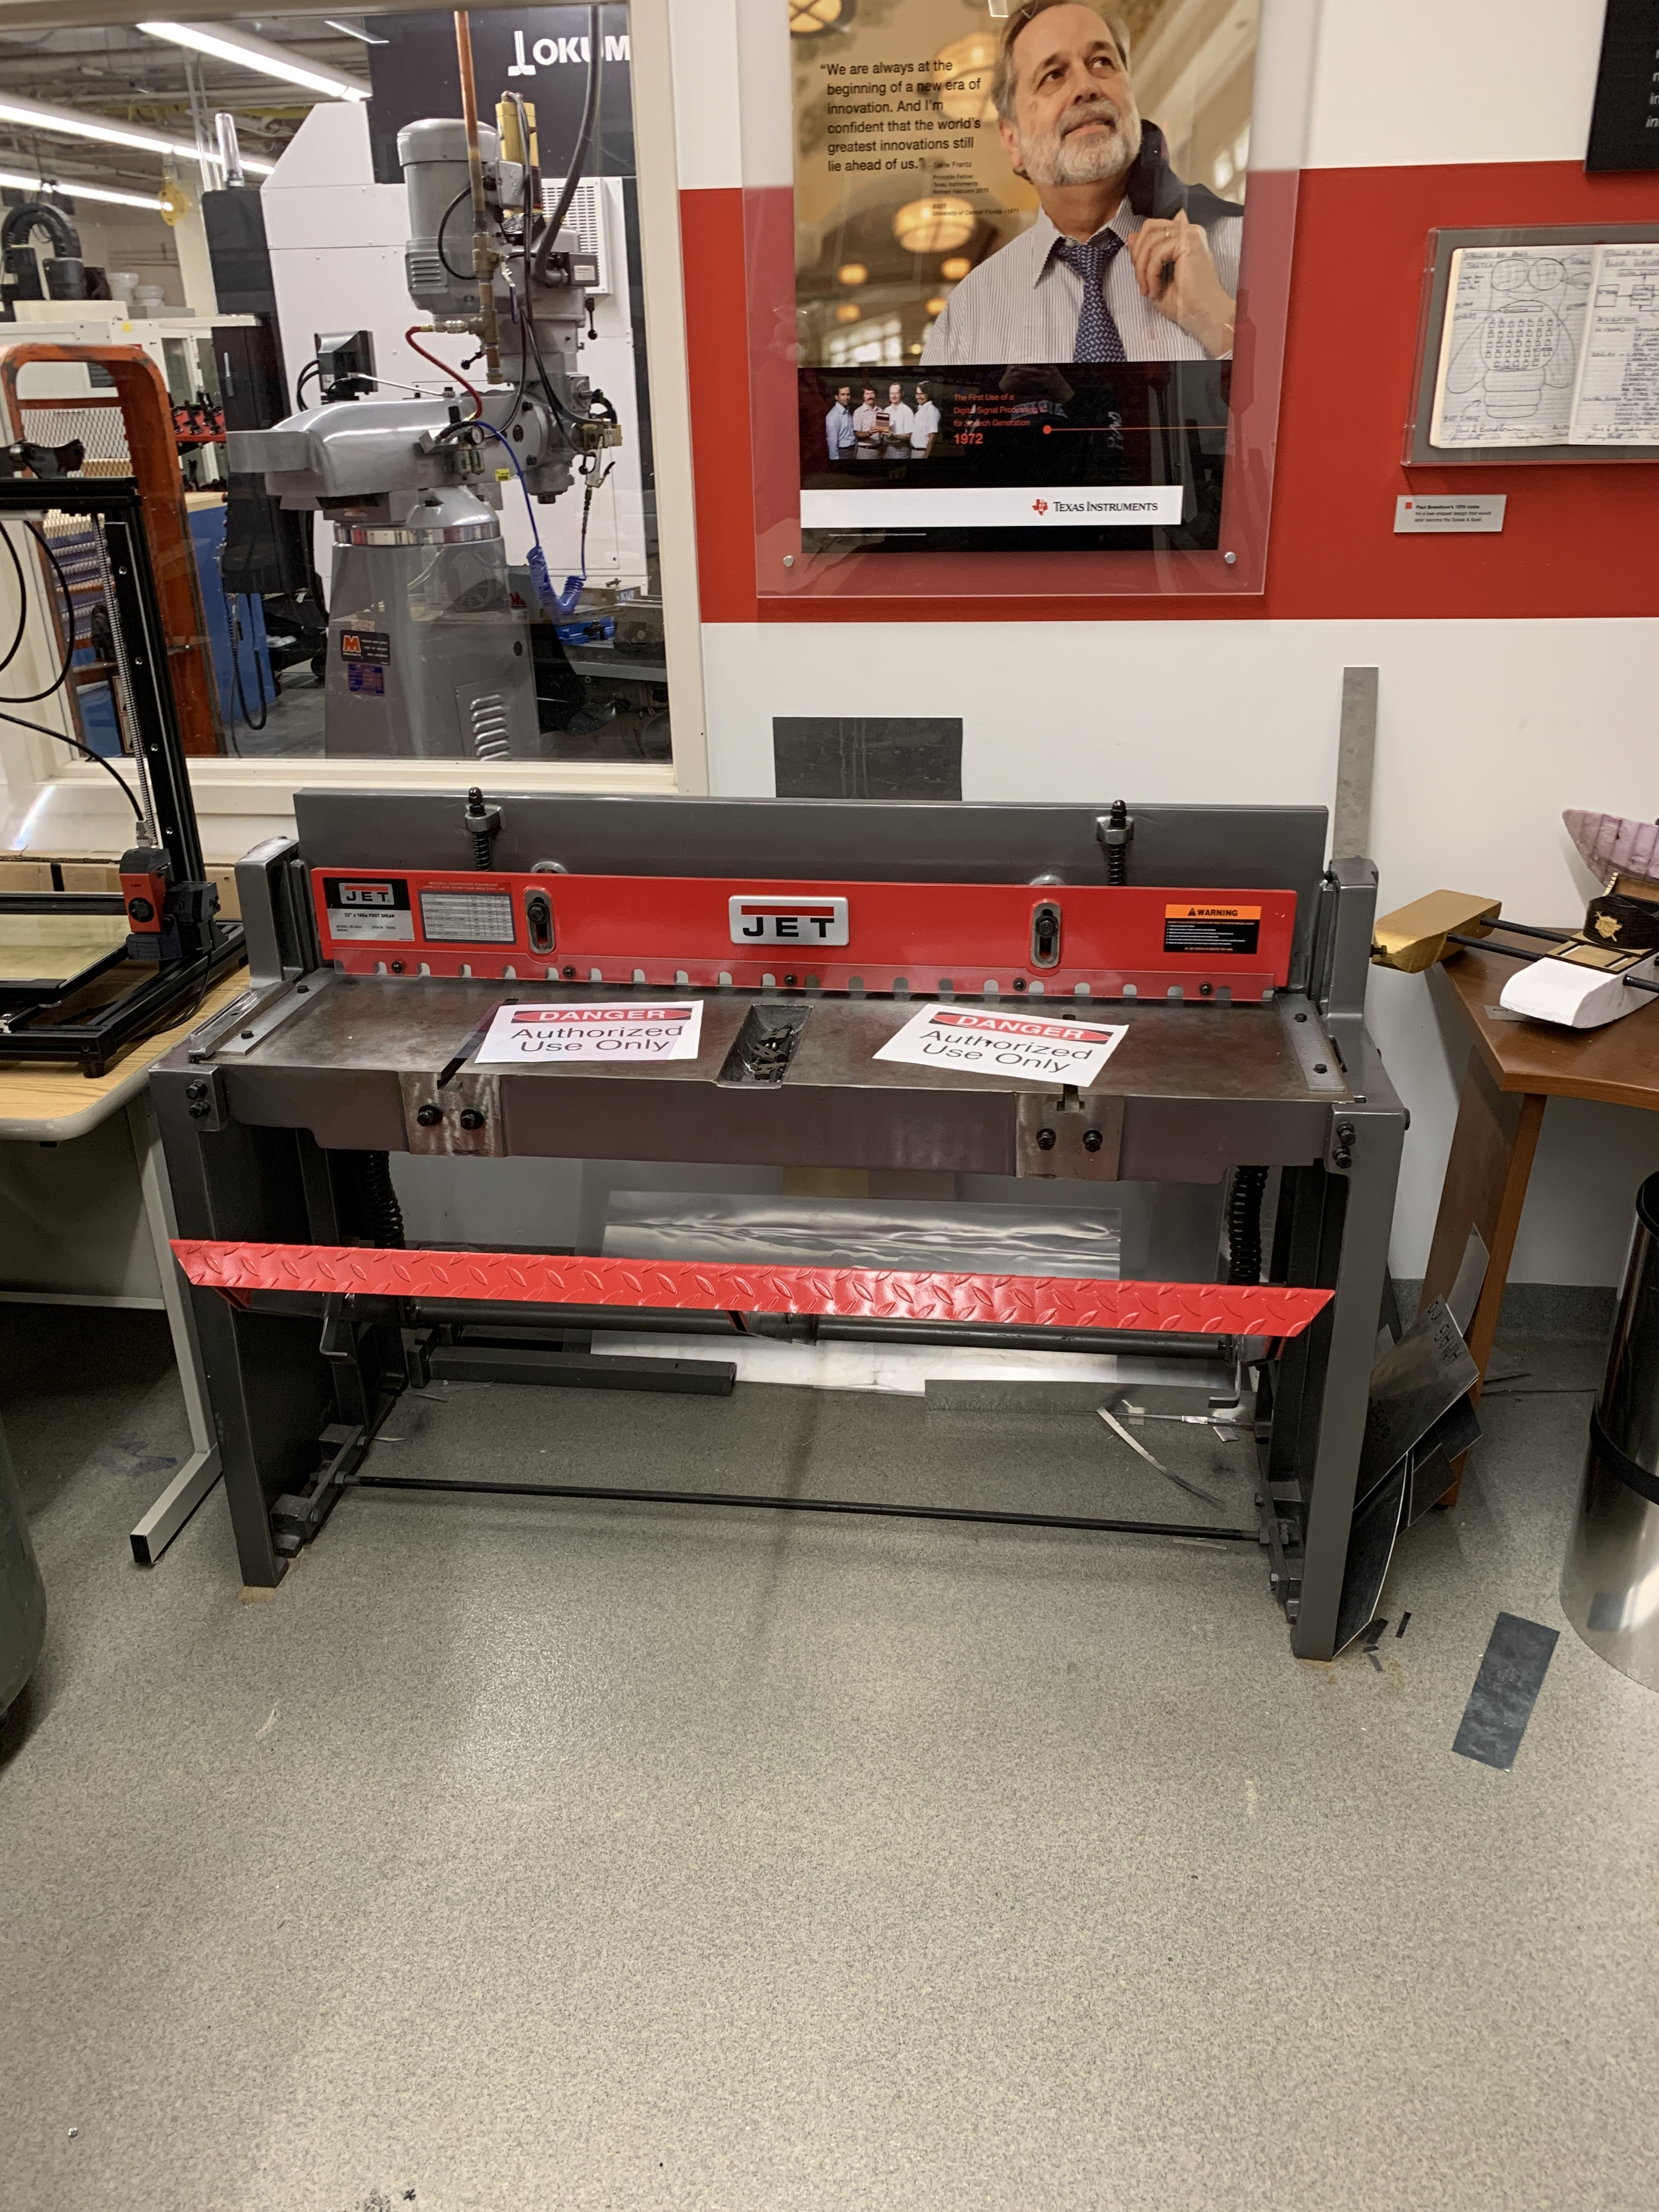
\includegraphics[width=0.95\textwidth]{Meetings/November/11-01-21/11-1-21_Hardware_Figure3 - Nathan Forrer.JPG}
  \caption{UCF Innovation Lab Shear}
  \label{fig:pic6}
\end{minipage}%
\hfill%
\begin{minipage}[b]{.48\textwidth}
  \centering
  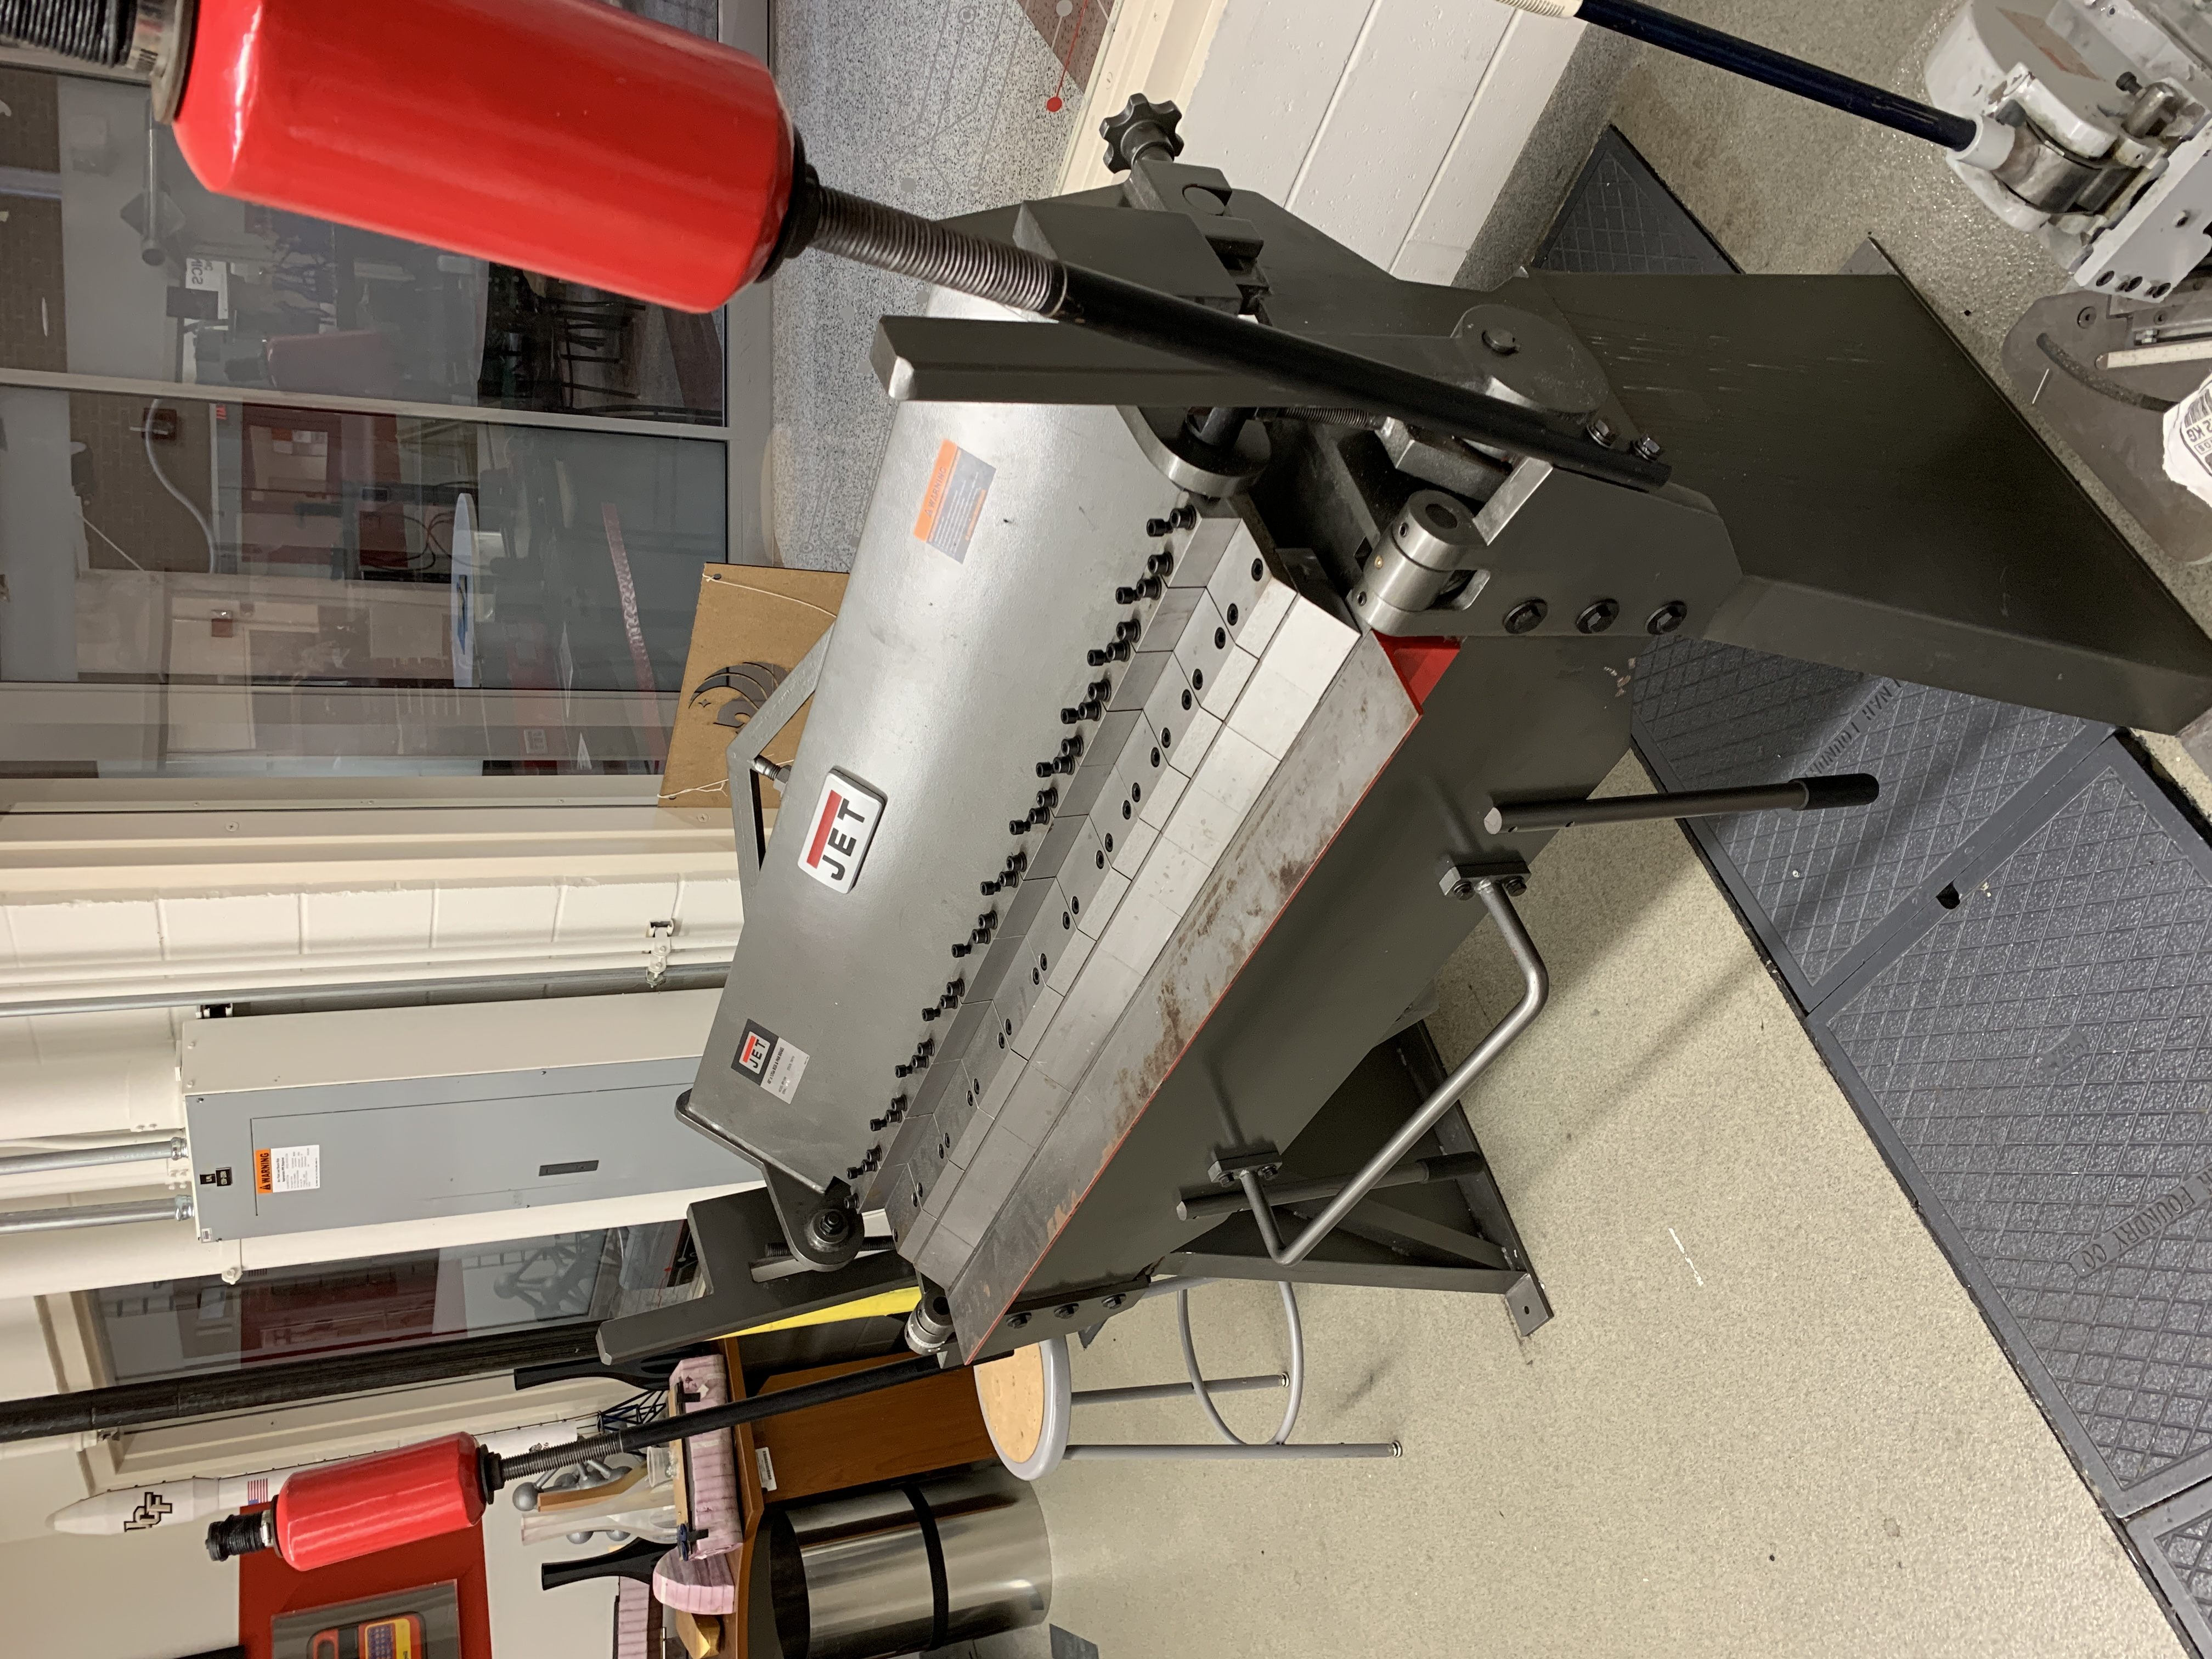
\includegraphics[width=0.95\textwidth]{Meetings/November/11-01-21/11-1-21_Hardware_Figure4 - Nathan Forrer.JPG}
  \caption{UCF Innovation Lab Brake}
  \label{fig:pic7}
\end{minipage}
\end{figure}

\begin{figure}[htp]
\centering
  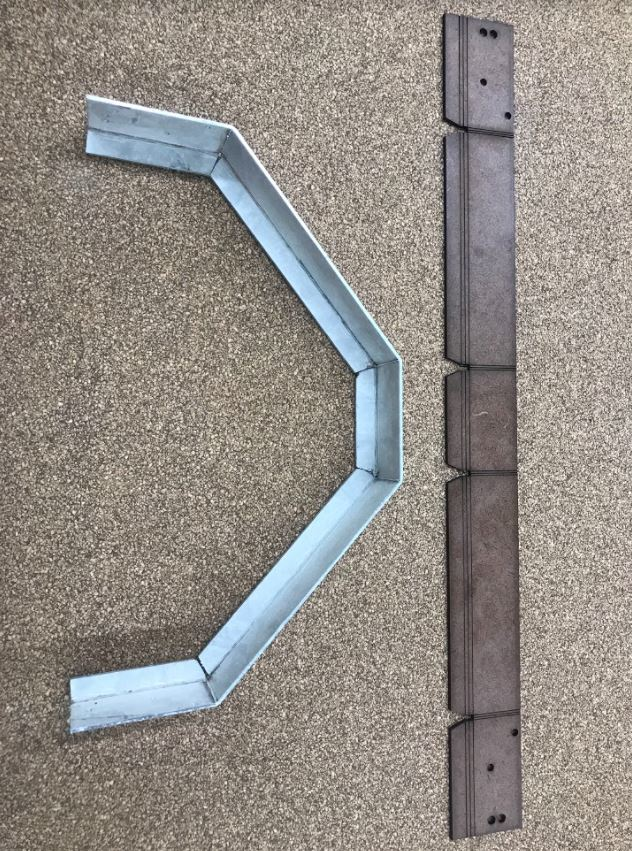
\includegraphics[width=0.95\textwidth]{Meetings/November/11-01-21/11-1-21_Hardware_Figure5 - Nathan Forrer.JPG}
  \caption{The finished bumper}
  \label{fig:pic8}
\end{figure}

\whatsnext{
\begin{itemize}
    \item Add bumper onto robot
    \item Test the robot in a scrimmage
    \item Work on making the arm stable
\end{itemize} 
}

